%% 
%% Copyright 2020 Ted Dunning
%% 
%% This document was created with reference to the SIMPA author guide but
%% is not a derived work under the terms of the LaTeX Project Public License (LPPL).

\documentclass[preprint,12pt, a4paper]{elsarticle}

%% Use the option review to obtain double line spacing
%% \documentclass[authoryear,preprint,review,12pt]{elsarticle}

%% For including figures, graphicx.sty has been loaded in
%% elsarticle.cls. If you prefer to use the old commands
%% please give \usepackage{epsfig}

\usepackage{amssymb}
\usepackage{hyperref}

% split long URLs in references
\usepackage{xurl}

% push figures to end
\usepackage[nomarkers,figuresonly]{endfloat}


%% The amsthm package provides extended theorem environments
%% \usepackage{amsthm}

%% The lineno packages adds line numbers. Start line numbering with
%% \begin{linenumbers}, end it with \end{linenumbers}. Or switch it on
%% for the whole article with \linenumbers.
%\usepackage{lineno}

\journal{Software Impacts}

\begin{document}

\begin{frontmatter}


 \title{The $t$-digest: Efficient Estimates of Distributions}


\author{Ted Dunning\corref{cor1}}
\ead{ted.dunning@gmail.com}
\ead[url]{http://tdunning.blogspot.com/}
\cortext[cor1]{Corresponding author}
\address{Hewlett Packard Enterprise, Los Altos, California}

\begin{abstract}
The $t$-digest is an on-line algorithm for building small sketches of data that can be used to approximate rank-based statistics with high accuracy, particularly near the tails.  This new kind of sketch is robust with respect to skewed distributions, repeated samples and ordered datasets. Separately computed sketches can be combined with little or no loss in accuracy.

An open-source Java implementation with no external dependencies of this algorithm is available as a free-standing library. Independent implementations in Go, C++ and Python are available. The $t$-digest is in widespread internal use in major companies and is also available in popular software such as Postgres, ElasticSearch, Apache Kylin and Apache Druid.

This research did not receive any specific grant from funding agencies in the public, commercial, or not-for-profit sectors.
\end{abstract}

\begin{keyword}
quantile estimation \sep t-digest \sep OLAP database \sep open-source \sep Greenwald-Khanna algorithm

\MSC[2020] 62G07 \sep 62G30 62P99 65D99 65Z99 
\end{keyword}

\end{frontmatter}

%\linenumbers
\section{Sketch Algorithms and Estimating Distributions}
Numerical data are often summarized using means, standard deviations, or using minimum or maximum values. This can give an idea of the central tendency of data but fails to give much information about the overall distribution. One particular virtue of such simple statistics is that they can be computed accurately  using a small amount of intermediate state.

Other interesting statistics are much more difficult to deal with. If we want to know the most common value, or the number of distinct values, or even just the median without sorting all of the data or making multiple passes through it, the best currently known approach is to compute a small summary of the data (called a digest or a sketch) and then use that summary to estimate the value we really want. For many such statistics, there is an unavoidable trade-off between the size of the digest and the accuracy of our estimates. The goal of research into sketching algorithms is all about trying to find ways to have smaller digests or sketches that give more accurate results while minimizing the effort to construct the sketch.

The $t$-digest is just such a data structure. As data is added, the $t$-digest maintains an estimate of the cumulative distribution function of the data seen so far. A $t$-digest can be used to estimate rank statistics such as the median, percentiles as well as trimmed means. Importantly, the $t$-digest can provide these statistics with orders of magnitude better accuracy than previous algorithms, particularly quantiles near 0 or 1, with very low amortized computational complexity. Moreover, $t$-digests can be pre-computed and later combined so that data can be summarized and explored in a highly interactive way.
\section{Why $t$-digest?}
The $t$-digest has become very popular. Based on personal communications, the $t$-digest is widely used in major companies such as Microsoft, Facebook and Google. It is also available as part of important software including Postgres \cite{postgres-t-digest}, ElasticSearch \cite{elastic, elastic-t-digest}, Apache Kylin \cite{kylin, kylin-t-digest}, and Apache Druid \cite{druid, druid-t-digest} and many others. For Postgres, ElasticSearch and Apache Druid, the $t$-digest works as an accumulator to allow percentiles of query data to be computed in a single parallel pass through selected data without large demands on memory. In Kylin, the integration is deeper. Much in the style of OLAP indexes in data warehouse systems, sketches of small subsets of data known as cubes are computed during index time and later combined at query time. Without this ability to pre-compute, store and later combine sketches, it would be impossible to apply OLAP principles to queries requiring the computation of rank-based statistics. The $t$-digest allows this to be done with much smaller indexes while achieving more accurate results. Both Postgres and Kylin are SQL based so the user view is similar. In Apache Kylin, for instance, there is a \texttt{percentile} function that can be used in SQL queries. Based on example queries, the system determines suitable cubes to support similar queries. Druid and ElasticSearch, on the other hand, each support their own idiosyncratic non-SQL syntax, but the principles are quite similar.

As of August, 2020, version 3.2 of the t-digest has over 1 million downloads / month from the central maven repository \cite{maven-stats} and has over a thousand stars on GitHub (unusually large for a statistical library).

The $t$-digest is not, however, the only way to estimate quantiles.  What distinguishes the $t$-digest is the ability to analyze data from an arbitrary distribution with better accuracy with a very small digest. Other quantile estimation algorithm fall roughly into the following categories:
\begin{itemize}
\item Sample selection algorithms such as the Greenwald-Khanna algorithm \cite{Greenwald-space-efficient-online-quantiles}. These algorithms retain a small number of the original samples that allow strong guarantees about the quantiles associated with these samples. Unfortunately, accurate information about the samples between the retained samples is difficult to retain with these algorithms so the resulting accuracy meets the guarantees, but not much more.
\item Clustering algorithms such as the $Q$-digest or the $t$-digest where a heuristic assignment of samples to so-called centroids is made. This clustering focus allows easy and accurate collection of means but the sample sets assigned to each centroid can overlap making it impossible to provide strong guarantees of accuracy. On the other hand, the $t$-digest uses the information collected about each centroid together with nearly correct assumptions about ordering of sample sets allows very good interpolation.
\item Fixed bin algorithms such as \texttt{Hdr\-Histogram}\cite{hdr-histogram}. These algorithms are useful when absolute or relative accuracy in the measurement space is most important (for instance when dealing with latencies). These algorithms are fast and have accuracy guarantees, but cannot be applied to general data distributions. Since the bin boundaries are fixed, compatible histograms can be accumulated precisely using vector addition. The $t$-digest library includes an optimized version of such a histogram known as the \texttt{LogHistogram}.
\end{itemize} 
\section{How to Use a $t$-digest}
Currently, there are several implementations available in the $t$-digest library. Of these, the \texttt{MergingDigest} implementation of a $t$-digest provides the best combination accuracy, size and amortized speed and requires no dynamic allocation after construction. Most insertions are very fast, but a compaction is done every few hundred or thousand samples that is slower. The \texttt{AVLTreeDigest} is nearly as good on accuracy but requires dynamic allocation, uses more memory and is a small factor slower, but it provides very consistent insertion times. 

Constructing a $t$-digest requires a compression parameter $\delta$ which determines the size of the digest and accuracy of quantile estimation. All other options can and almost always should be left at default settings. The scaling of accuracy versus $\delta$ is illustrated in Figure \ref{fig:accuracy-scaling}.
\begin{figure}[htb] %  figure placement: here, top, bottom, or page
   \centering
   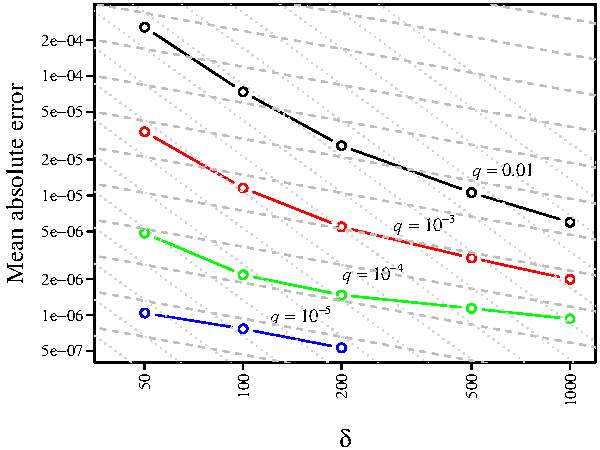
\includegraphics[width=4in]{figures/error-vs-compression.pdf} 
   \caption{The scaling of quantile estimation for various values of compression factor $\delta$ and $q$ for $10^6$ samples. 
   The general pattern is that absolute error scales like $1/\delta^2$ for small values of $\delta$ and like $1/\sqrt{\delta}$ for values larger than some cutoff. The cutoff is higher for larger values of $q$ (roughly 500 for $q=0.01$ but only 100 for $q=10^{-5}$). The grey dashed lines provide a reference for $1/\sqrt{\delta}$ scaling, the dotted grey lines show $1/\delta^2$.   At $q=10^{-5}$ error goes to zero for values $\delta > 200$ and cannot be shown on a log scale. The same happens for $q=10^{-6}$ except error is zero for all values of $\delta$. }
   \label{fig:accuracy-scaling}
\end{figure}

In a monitoring or query application, it is typical to build digests for each kind of measurement for short time windows (typically a few minutes in length) and then store these digests. Later when a data visualization or query is done, these windowed digests can be combined and displayed as needed.  Since $t$-digests can be added together as needed, this architecture allows a broad range of queries to be satisfied. This is how Apache Kylin\cite{kylin} and Apache Druid\cite{druid} use the $t$-digest. 

The Kylin use-case is particularly interesting since the digest is integrated into a full OLAP data warehouse system. Postgres\cite{postgres-t-digest}, in contrast, uses the $t$-digest in a more limited way to speed up queries involving approximate quantiles. The benefit with Kylin and Druid is a dramatic apparent speedup that comes about because most of the work of creating digests is done during data ingestion rather than at query time thus eliminating the need to scan (or even to store) the raw data for queries involving rank-based statistics. With Postgres there is a smaller (but still very significant) benefit in terms of memory usage and speedup that comes from the fact that the necessary $t$-digest can be constructed in a single parallelized pass through the data as opposed to requiring that the raw data be sorted.

Another common use of $t$-digests is as a final processing step in anomaly detection\cite{anomaly-detection}. The idea is that the anomaly detection system contains a model of some kind that outputs a score that is higher when anomalous conditions are present. This score is then compared to a threshold and an alarm is raised if the score is above the threshold. This threshold, however, is stated in terms of the anomaly model and is not easily understood by users. As such, it is desirable to allow users to set the threshold in terms of the rate of alarms that can be handled. To do this, it is typical to accumulate $t$-digests for time windows and then combine recent windows to get a digest that actually computes the threshold as shown in \ref{fig:window-thresholds}. As new window digests become available, new combined digests can be computed in a rolling fashion. This process is illustrated in Figure \ref{fig:window-thresholds}. The threshold can then be set in terms of a quantile from the historical data. This is translated into a threshold by the digest.
\begin{figure}[htb] %  figure placement: here, top, bottom, or page
   \centering
   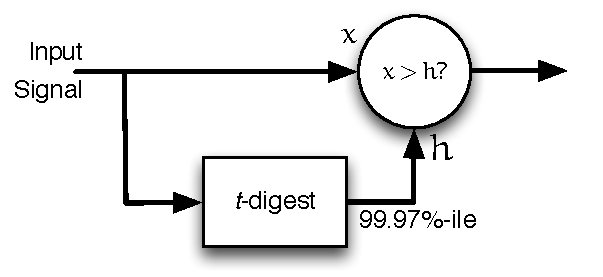
\includegraphics[width=3in]{figures/adaptive-threshold.pdf} 
   \caption{
Users can set thresholds in terms of score quantiles instead of scores by using a $t$-digest.}
   \label{fig:adaptive-thresholds}
\end{figure}
\begin{figure}[htb] %  figure placement: here, top, bottom, or page
   \centering
   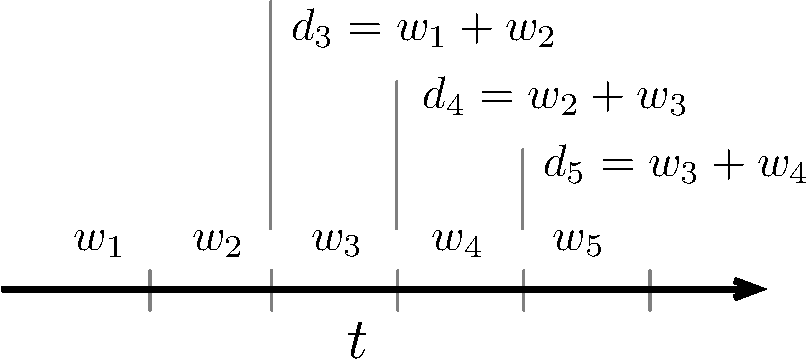
\includegraphics[width=3in]{figures/windows.pdf} 
   \caption{
   Thresholds for anomaly detection can be computed by combining digests for individual time windows. Digests $w_1 \ldots w_5$ are computed for each window as data arrives and are persisted when the window ends. For computing thresholds, combined digests $d_3$, $d_4$ and $d_5$ are computed as soon as a window ends and define the alarm threshold during their life. If smooth changes in threshold levels are desired, threshold levels can be interpolated between old and new digests during a short transition period.}
   \label{fig:window-thresholds}
\end{figure}


In contrast to monitoring for extreme values in anomaly detection, some systems require looking for changes in a score distribution\cite{machine-learning-logistics}. This is typical with decisioning systems based on machine learning that are intended to detect, for instance, fraud. Substantial changes in the score distribution for small fraction of the highest scores can indicate a new kind of attack or important changes in overall user behavior that indicates a new model should be trained and deployed. To detect this kind of change, a digest can be constructed for a reference time period. This reference digest can generate thresholds for score ranges and a digest for the current period can be used to compute counts for the number of scores that fall into these ranges during the current period. These counts can be compared to the number of scores that fell into those ranges during the reference period using $\chi^2$ tests such as the $G^2$ test\cite{dunning93}.


\section{Research and Industrial Impact}
The $t$-digest is primarily used in monitoring and data exploration software and has largest impact in industrial settings where efficient monitoring can make a large difference due to early detection and (hopefully) mitigation of malfunctions. The $t$-digest enables data to treated as a distribution as opposed to simpler statistics such as a mean or extreme values. This change in view from point estimate to distribution has practical impact because performance of many systems is difficult to understand without knowing something about the distribution of data. System response latency is a classic example of this\cite{tene}. With latencies, one common method for analysis is to set breakpoints at the 95, 99, and 99.9 percentiles for the historically observed distribution of latencies. Short-term counts for latencies falling into the ranges defined by these breakpoints can then be analyzed using $\chi^2$ statistics using the same method as was described in the previous section for analyzing the distribution of scores for machine learning models.

Another example arises any time that more measurements are made than can be stored leading to a desire to at least retain information about the distribution of the measurements for a particular time period. The common virtue of the $t$-digest in all of these cases is that a single technique can reduce data to a small sketch while retaining accurate distributional information.

Where there is strong prior information about the distribution of data (as is typically the case with latencies, for example), then special purpose algorithms such as the \texttt{HdrHistogram} or the \texttt{LogHistogram} can be useful, but where such information is not known, the $t$-digest provides a generally superior trade-off between generality (because it handles any distribution equally well) and accuracy (because it interpolates well). In many cases, even if a good prior is available, it is more convenient to use the $t$-digest since it has been integrated into so many systems already and the cost of its generality is low (typically less than 2:1 relative to \texttt{LogHistogram}, for instance).

Monitoring the output of machine learned models is another good example of the use of a $t$-digest. The distribution of these outputs is often a very good indicator of whether the model is working as expected and the $t$-digest makes it easy to test for changes in this distribution. Comparing the distribution of new model output  against the historical outputs allows very simple change point detection\cite{machine-learning-logistics, anomaly-detection}. Detecting these change points allows better accuracy since new models can be built at a slower cadence, yet be deployed sooner after large behavioral changes. Figure \ref{fig:change-point} shows how this technique works on synthetic data where only 20 data points out of 1000 per test period come from a shifted distribution. For this test, cut points were set at the 99-th and 99.9-th percentiles resulting in four counts per time period to be compared to a comparable set of counts from a reference period. These counts were compared using a log-likelihood ratio test as described in \cite{dunning93}
\begin{figure}[htb] %  figure placement: here, top, bottom, or page
   \centering
   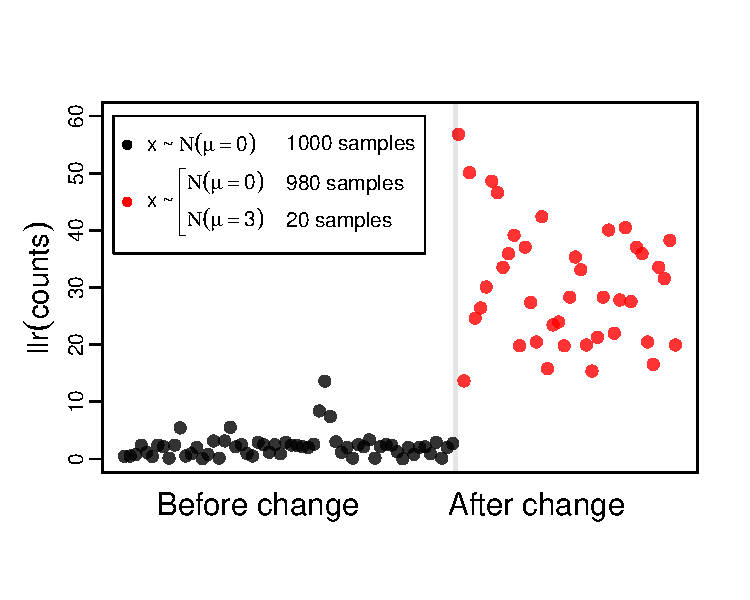
\includegraphics[width=3in]{figures/change-point.pdf} 
   \caption{
   Even very small changes in the distribution of points can be detected robustly. Here, only 20 samples out of 1000 per sample period are perturbed, but a $\chi^2$ test applied to counts derived from distributional information detects the change reliably. The bin boundaries here were set to the 99th and 99.9th empirical percentiles of the signal in a reference period.}
   \label{fig:change-point}
\end{figure}
The code used to generate the data in this figure is available \cite{shift-detection}.

The authors have observed that the benefits of the $t$-digest so far accrue dominantly to industrial applications as opposed to research projects because industrial settings often have clear economic rewards for efficient monitoring since that can allow high uptime. For most research applications, ongoing monitoring efficiency is not an issue and many research datasets are small enough that sorting the entire dataset in memory to compute rank-based statistics is not a significant penalty. There are a few research areas, however, where such monitoring or the reduction of query times against very large datasets is of primary concern. For instance, internet observatories looking for and analyzing signs of large-scale cyber-attacks can benefit from large scale characterization of the distributions of various metrics.

In general, understanding distributions of data allows more nuanced decision making through better human understanding and through more expressivity in automated systems. With the $t$-digest, recording and analyzing distributions is not much more difficult than computing a mean or standard deviation which makes these potential improvements much more accessible.

\section*{Declaration of Competing Interest}
The author declares that he has no competing financial interests or personal relationships that could have appeared to influence the work reported in this paper.
\section*{Acknowledgements}

I would like to thank all of the contributors to the $t$-digest. These notably include Adrien Grand for the implementation of the AVLTreeDigest and Otmar Ertl whose contributions led to the current formulation of the scale function. Non-code contributions should be recognized such as the efforts by 
Cameron Davidson-Pilon to explain and popularize the $t$-digest\cite{cameron-t-digest}. Lastly, everyone who has used the $t$-digest or commented on it has helped improve it.

As with all open source software, these people make up the community around the $t$-digest and it is the community that breathes life into otherwise lifeless code. Thank you all.

%% The Appendices part is started with the command \appendix;
%% appendix sections are then done as normal sections
%% \appendix

\bibliographystyle{elsarticle-num} 
\bibliography{refs.bib}


\begin{table}[!h]
\begin{tabular}{|l|p{5cm}|p{8cm}|}
\hline
\textbf{Nr.} & \textbf{Code metadata description} & \textbf{Value} \\
\hline
C1 & Current code version &3.2 \\
\hline
C2 & Permanent link to code/repository used for this code version & \url{https://github.com/tdunning/t-digest} \\
\hline
C3  & Permanent link to Reproducible Capsule & \url{https://doi.org/10.24433/CO.6606319.v1} \\
\hline
C4 & Legal Code License   & Apache License 2.0 \\
\hline
C5 & Code versioning system used & git \\
\hline
C6 & Software code languages, tools, and services used & Java \\
\hline
C7 & Compilation requirements, operating environments & JDK 8 or higher  \\
\hline
C8 & If available Link to developer documentation/manual & \url{https://github.com/tdunning/t-digest/blob/master/README.md} \\
\hline
C9 & Support email for questions & ted.dunning@gmail.com  \\
\hline
\end{tabular}
\caption{Code metadata}
\label{metadata} 
\end{table}

\end{document}
\endinput
%%
%% End of file `SoftwareX_article_template.tex'.
